\chapter{Prototype implementation}\label{chap:impl}

\section{Programming discipline}
The prototype was implemented largely in the spirit of exploratory programming:
``the kind where you decide what to write by writing
it.''\cite{arc}.

This approach in combination with a dynamic and flexible language like
JavaScript enables one to quickly transform ideas to working prototypes and
shape them as one goes along. But the usefulness of this method is limited, as
it may quickly produce fairly low-quality code, as it is not focused on future
maintainability.

Most of the features of the language and editor in the prototype are implemented
as a proof-of-concept, although some are more refined than others in order to
fulfil the major goals of this thesis, one of which was to implement a working
non-trivial application in the language.

\section{The language}
The prototype implementation of the language contains all the features described in Chapter \ref{chap:lang}, with the following exceptions:
\begin{itemize}
    \item Macros are not implemented.\footnote{In fact, they partially \textit{are} implemented, but are not usable. For example, there is a \texttt{macro} primitive available, which produces macro values. But it should not be used, as these macro values are not treated specially by the interpreter, so using them will not have the desired effect.}
    \item There are two primitives, which produce function values: \texttt{of} and \texttt{of-p}. The second has the same meaning as \texttt{of} described in Chapter \ref{chap:lang}. The first has the same meaning, except that it does not use pattern matching when binding names to arguments. This primitive requires that all the names must be words.
    \item Destructuring is not implemented for assignments (it does not work in \texttt{mutate}), only for definitions (it works in \texttt{bind}). Pattern matching could easily be extended to mutation, although I have found it sufficient to be usable only in definitions and ended up not implementing it for assignments in the prototype.
    \item Comments are treated as a streams of characters, taking into account nesting and balancing of brackets in multi-line comments, but are not preserved on the \acrshort{est} as a tree-like structure.
    \item Strings are not recognized specially by the parser. They are stored and manipulated as syntax tree nodes, not as streams of characters. This means that the optimization described in Section \ref{sub:str} was not applied. The performance penalty is acceptable in the prototype implementation. 
    \item The escape character \texttt{\\} has no special meaning. To substitute a special character in a string, the following built-in values are defined:
    \begin{lstlisting}
    (left-bracket) -- escapes "["
    (right-bracket) -- escapes "]"
    (left-brace) -- escapes "{"
    (right-brace) -- escapes "}"
    (pipe) -- escapes "|"
    (bang) -- escapes "!"
    \end{lstlisting}
    
    So \texttt{'[(left-bracket)hello(right-bracket)]} would evaluate to: \texttt{"[hello]"}.
\end{itemize}

Lisp's syntax is as minimal as it gets\cite{syntaxation}, which makes 

An interpreter for Lisp is also trivial to implement, so this is a good starting
point.

There are many approaches to implementing interpreters for LISP in
JavaScript\cite{js_lisps}, but the general principles are the same.

\subsection{Macros}
This
macro system is not included in the final version of the prototype, although a
proof-of-concept of it that I implemented in earlier prototypes


One feature that I experimented with while creating the prototype of Dual is
support for first-class just-in-time expanded macros

\section{The environment}

The goal is to build an online \acrlong{ide} IDE, similar to
Codeanywhere\cite{codeanywhere_website} or
Cloud9\cite{c9_website}, which works offline as well.

\section{Performance}
It could be optimized similarly to CodeMirror or other web-based text editors or
applications. That is, only a visible portion (plus a margin, which allows for
fast scrolling) of the code is rendered as DOM nodes at any time. The scrollbar
is virtual and controlled by the editor rather than the browser.

Text editors like CodeMirror use similar amount of DOM nodes [[]], but thanks to
these optimizations are able to handle
megabyte-sized\cite[Section~General Approach]{cm_internals}
text files and are used in many real-world
applications\cite{cm_realworld}, which
includes being a built-in editor in developer tools in major web browsers.

Another source of inefficiency is that parsing is done twice -- once by Dual's
parser and once by CodeMirror's system, which are incompatibile.  A solution to
that would be to implement a custom text editor or extend/modify CodeMirror to
work with Dual's parser.


\begin{figure}[h!]
\centering 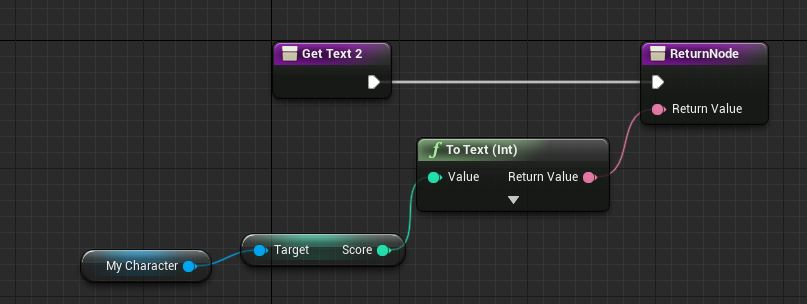
\includegraphics[width=0.9\textwidth]{blueprint}
\caption{
    Blueprints Visual Scripting;
    screenshot from \protect\cite{fig_blueprint2}
}
\label{fig:blueprint2}
\end{figure}


